\chapter{Future Work}

This research merely scratches the surface, and vast territories are yet uncharted. In future studies, the following areas will be explored to extend the current research further:

\begin{itemize}
  \item Investigate the effect of different transformations and augmentation pipelines. Incorporating track stems and different takes of the same piece as natural, human-made augmentations could yield interesting results.
  \item Expand input data to include dB-scale Mel-spectrum magnitude and CQT of audio. This approach has been widely used in music-related tasks with CNNs \cite{Kim2020OneStrategies}. Though raw audio provides a rich representation, dB-scale Mel-spectrum offers a frequency-domain summarization that is not only grounded in psycho-acoustics but is also computationally efficient and hard to reproduce solely through data-driven methods \cite{Kim2020OneStrategies}. Therefore, this trade-off is worth exploring.
  \item Implement k-fold cross-validation to improve the robustness of the model's performance.
  \item Experiment with different hyperparameters. For instance, setting the kernel size to $0.005$ times the sample rate could match the Just Noticeable Difference (JND). As for the loss function margin, a starting point of 0.2 has proven effective, but different values should be explored to optimize performance on the validation set.
  \item Increase the size of the representation layer to 512 or 1024 dimensions.
  \item Apply easy triplet mining to improve the model's performance \cite{XuanImprovedMining}.
  \item Implement visual and auditory evaluations: 2D or 3D visualization of the latent space \ref{fig:manifold}, coupled with a Graphical User Interface (GUI) that enables playback for evaluation, can help assess the extent to which the model considers sonic attributes. It would also facilitate the understanding of the clustering of complex musical content. 
\end{itemize}

\begin{figure}[ht]
    \centering
    \scalebox{1.2}{

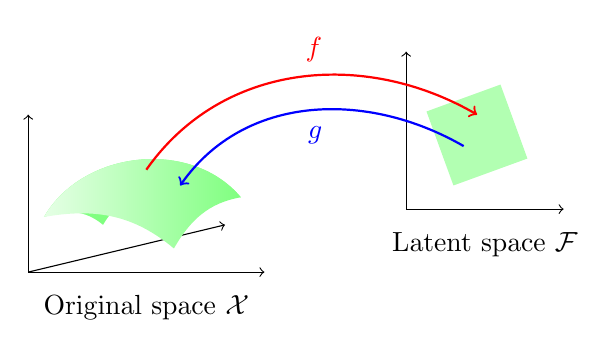
\begin{tikzpicture}
\centering
\draw[->] (0, 0) -- ++(0, 2);
\draw[->] (0, 0) -- ++(2.5, 0.6);
\draw[->] (0, 0) -- ++(3, 0) node[midway, below, yshift=-0.5em]
    {Original space ${\cal X}$};

\draw[fill=green!50, draw=none, shift={(0.2, 0.7)},scale=0.5]
  (0, 0) to[out=20, in=140] (1.5, -0.2) to [out=60, in=160]
  (5, 0.5) to[out=130, in=60]
  cycle;

\shade[thin, left color=green!10, right color=green!50, draw=none,
  shift={(0.2, 0.7)},scale=0.5]
  (0, 0) to[out=10, in=140] (3.3, -0.8) to [out=60, in=190] (5, 0.5)
    to[out=130, in=60] cycle;

  \draw[->] (4.8, 0.8) -- ++(0, 2);
  \draw[->] (4.8, 0.8) -- ++(2, 0) node[midway, below, yshift=-0.5em]
      {Latent space ${\cal F}$};

  \draw[thin, fill=green!30, draw=none, shift={(5.4, 1.1)}, rotate=20]
    (0, 0) -- (1, 0) -- (1, 1) -- (0, 1) -- cycle;

  \draw[thick,->,red]
    (1.5, 1.3) to [out=55, in=150] node[midway, above, xshift=6pt, yshift=2pt]
    {$f$} (5.7, 2);

  \draw[thick,->,blue] (1.5, 1.3) ++(4.03, 0.3) to [out=150, in=55]
    node[midway, below, xshift=2pt, yshift=-2pt] {$g$} ++(-3.6, -0.5);

\end{tikzpicture}}
    
    \caption[Dimensionality reduction and latent space representation \cite{tikz}.]{\small{Dimensionality reduction and latent space representation: Mapping between the original high-dimensional space ${\cal X}$ and the lower-dimensional latent space ${\cal F}$ using functions $f$ and $g$.}}
    \label{fig:manifold}
\end{figure}


\newpage